\documentclass[12pt]{article}

\usepackage[T2A]{fontenc}
\usepackage[utf8]{inputenc}
\usepackage[russian]{babel}

\usepackage{mathtext}
\usepackage{cmap}
\usepackage{amsmath,amssymb,amsthm,amscd,amsfonts}
\usepackage{graphicx}
\usepackage[colorbox,usenames,dvipsnames]{xcolor}
\usepackage{float, caption, subcaption, multirow}
\usepackage[section]{minted}
\usepackage{hyperref}

\voffset -24.5mm
\hoffset -5mm
\textwidth 173mm
\textheight 240mm
\oddsidemargin=0mm \evensidemargin=0mm

\definecolor{codegray}{gray}{0.9}
\newcommand{\code}[1]{\colorbox{codegray}{\texttt{#1}}}
\newmintinline[src]{console}{}

\renewcommand{\theFancyVerbLine}{\sffamily\textcolor{black}{\scriptsize\oldstylenums{\arabic{FancyVerbLine}}}}
\usemintedstyle[console]{bw}
\setminted[console] {
     bgcolor = codegray,
     linenos = true,
     tabsize = 2,
     formatcom = \color{black},
     frame = leftline,
     framerule = 0.8pt,
     framesep = 0.5cm,
     xleftmargin = 1cm,
     breaklines = true,
     escapeinside=||
}

\begin{document}

\title{
    Лабораторная работа №1 \\ 
    Дисциплина <<Методы и средства защиты информации>> \\ 
    GPG}
\author{Евгений Хандыго, гр. 53501/3}

\maketitle
\tableofcontents

\newpage

\section{Постановка задачи}

В рамках данной работы необходимо овладеть основными аспектами работы с утилитой gpg4win. Ход работы соответствует следующим пунктам:
\begin{itemize}
    \item Изучить документацию gpg и gpg4win.
    \item Поставить собственную ЭЦП на файл.
    \item Проверить ЭЦП на стороннем файле.
    \item Обменяться зашифрованными сообщениями с другим пользователем gpg.
    \item Потренироваться в использовании утилиты gpg через интерфейс командной строки.
\end{itemize}
\section{Поставить собственную ЭЦП на файл}

Для того, чтобы начать работать с gpg, сначала необходимо сгенерировать собственную пару ключей, состоящую из публичной (сертификат)
и приватной частей. Публичный ключ может распространяться свободно (в том числе и в сети Интернет), в то время как передача
приватного ключа третьим лицам категорически запрещена. Для того, чтобы сгенерировать пару ключей с помощью  gpg необходимо 
воспользоваться опцией \src{--gen-key}. Пример вывода утилиты gpg при использовании данной опции представлен ниже в листинге 
\ref{lst:gen-key}. 
\\ \hfill \\
\inputminted[lastline=23]{console}{resources/01_gen_key}
\inputminted[firstline=25]{console}{resources/01_gen_key}
\captionof{listing}{Вывод утилиты gpg при вызове с опцией \src{--gen-key} \label{lst:gen-key}}

\begin{figure}[H]
    \centering
    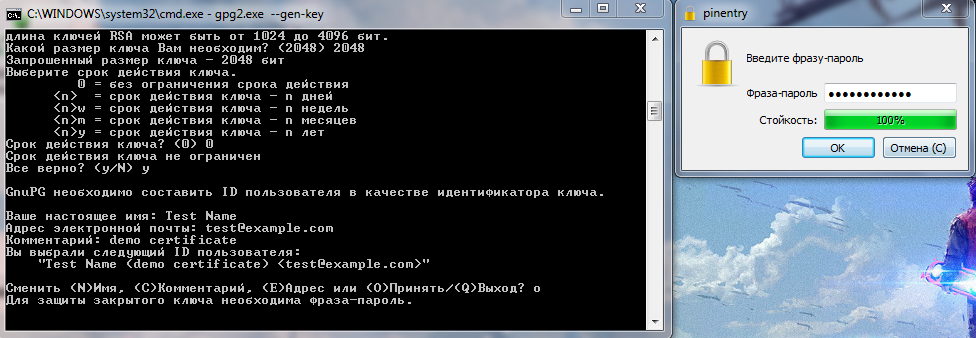
\includegraphics[width=16cm]{resources/02_gen_key.png}
    \caption{Форма ввода пароля при генерации ключей в gpg}
    \label{fig:gen-key-password-form}
\end{figure}

При этом в строке $34$ вывода происходит предоставление пользователю формы для ввода пароля генерируемого приватного ключа. В случаях,
когда приватный ключ скомпрометирован, данный пароль является последней ступенью защиты перед злоумышленниками. Форма ввода пароля
показана на рисунке \ref{fig:gen-key-password-form}. После ее ввода требуется также подтверждение выбранного пароля.

Для дальнейшего использования созданных ключей необходимо сначала экспортировать свой сертификат для того, чтобы его можно было 
передать лицам, заинтересованным в отправке зашифрованных и/или подписанных сообщений пользователю. Для этого необходимо 
воспользоваться опцией \src{--export}. Дополнительно также можно использовать опции \src{--armor}, которая преобразовывает вывод из 
бинарного формата в формат ASCII, и \src{--output} для указания файла записи результата. Пример вызова утилиты gpg с опцией 
\src{--export} представлен в листинге \ref{lst:export-certificate}.

\begin{listing}[H]
    \inputminted[lastline=14]{console}{resources/03_export_certificate}
    \caption{Вывод утилиты gpg при вызове с опцииями \src{--export} и \src{--armor}}
    \label{lst:export-certificate}
\end{listing}

Одним из основных сценариев использования утилиты gpg --- это установка электронной цифровой подписи. Для установки ЭЦП на какой-либо
файл необходимо воспользоваться опцией \src{--sign} или \src{--detach-sign} как показано в листинге \ref{lst:sign-file}.

\begin{listing}[H]
    \inputminted{console}{resources/04_sign_file}
    \caption{Вывод утилиты gpg при вызове с опцией \src{--detach-sign}}
    \label{lst:sign-file}
\end{listing}

После выполнения этой команды будет создан отдельный файл цифровой подписи. Его содержание представлено в листинге \ref{lst:file-sign}

\begin{listing}[H]
    \inputminted{console}{resources/05_file_sign}
    \caption{Пример цифровой подписи}
    \label{lst:file-sign}
\end{listing}
\section{Проверить ЭЦП на стороннем файле}

Для демонстрации проверки подлинности ЭЦП с помощью утилиты gpg были скачаны следующий файлы:
\begin{itemize}
    \item Инсталятор \href{https://files.gpg4win.org/gpg4win-vanilla-2.3.0.exe}{Gpg4win-Vanilla 2.3.0}.
    \item \href{https://files.gpg4win.org/gpg4win-vanilla-2.3.0.exe.sig}{Его цифровая подпись}.
    \item \href{https://ssl.intevation.de/Intevation-Distribution-Key.asc}{Сертификат}, с помощью которого была сделана подпись.
\end{itemize}
Теперь необходимо импортировать полученный сертификат. Для этого предназначена опция \src{--import}. Результат вывода утилиты gpg
при использовании данной опции представлен в листинге \ref{lst:import-certificate}.

\begin{listing}[H]
    \inputminted{console}{resources/06_import_certificate}
    \caption{Вывод утилиты gpg при вызове с опцией \src{--import}}
    \label{lst:import-certificate}
\end{listing}

Для дальнейшего использования импортированного сертификата необходимо подтвердить его полномочия (подписать). Согласно общепринятому 
мнению, данный этап подтверждения является Ахиллесовой пятой gpg, поскольку пользователь системы должен быть на сто процентов
уверен в личности создателя сертификата. Для решения данной проблемы рекомендуется проводить личные встречи с автором сертификата,
однако на практике, как правило, ограничиваются сверкой отпечатков сертификата. Также стоит отметить, что здесь имеет место быть 
концепция web of trust, согласно которой, получаемый сертификат уже может содержать определенное количество подписей от других 
пользователей. Это позволяет судить о степени доверия полученному сертификату по количеству других пользователей, которые подписали
его. Для того, чтобы подтвердить полномочия некоторого сертификата необходимо запустить утилиты gpg с опцией \src{--edit-key}
и затем ввести команду \src{sign}. Пример выполнения данной операции представлен в листинге \ref{lst:sign-certificate}.

\begin{listing}[H]
    \inputminted{console}{resources/07_sign_certificate}
    \caption{Вывод утилиты gpg при вызове с опцией \src{--edit-key}}
    \label{lst:sign-certificate}
\end{listing}

Для проверки электронной подписи теперь достаточно вызывать утилиту gpg с опцией \src{--verify} как показано в листинге 
\ref{lst:verify-sign}.

\begin{listing}[H]
    \inputminted{console}{resources/08_verify_sign}
    \caption{Вывод утилиты gpg при вызове с опцией \src{--verify}}
    \label{lst:verify-sign}
\end{listing}
\section{Обменяться зашифрованными сообщениями с другим пользователем gpg}

Для демонстрации передачи сообщений зашифрованных с помощью gpg был получен, импортирован и подписан сертификат другого пользователя 
gpg. Для подтверждения этого рассмотрим вывод утилиты gpg, запущенной с опцией \src{--list-keys}, представленный в листинге 
\ref{lst:keys-list}. Испортированный ключ соответствует пользователю \src{Sergey Klimov (Lab3) <ksa1993@yandex.ru>}.

\begin{listing}[H]
    \inputminted{console}{resources/09_keys_list}
    \caption{Вывод утилиты gpg при вызове с опцией \src{--list-keys}}
    \label{lst:keys-list}
\end{listing}

Для шифрования и подписи некоторого файла необходимо вызвать утилиту gpg с опциями \src{--sign} и \src{--encrypt}, а также 
с помощью опций \src{--local-user} и \src{--recipient} указать идентификатор сертификатов отправителя и получателя соответственно.
Пример вывода утилиты при шифровании файла указан в листинге \ref{lst:encrypt-file}. При этом, после вызова приведенной команды
будет создан greeting.txt.gpg, содержащий зашифрованные данные и электронную цифвровую подпись.

\begin{listing}[H]
    \inputminted{console}{resources/10_encrypt_file}
    \caption{Вывод утилиты gpg при вызове с опциями \src{--encrypt} и \src{--sign}}
    \label{lst:encrypt-file}
\end{listing}

Пересылка файла и его рассшифровка получателем прошли успешно.

Описанная выше операция по пересылке шифрованного сообщения была также в точности повторена со сменой ролей получателя и отправителя.
От другого пользователя gpg был получен зашифрованный файл pic.jpg.gpg, который был расшифрован с помощью опции \src{--decrypt} 
утилиты gpg, как показано в листинге \ref{lst:decrypt-file}. Расшифрованный файл представлен на рисунке \ref{fig:decryption-result}.

\begin{listing}[H]
    \inputminted{console}{resources/11_decrypt_file}
    \caption{Вывод утилиты gpg при вызове с опциями \src{--decrypt}}
    \label{lst:encrypt-file}
\end{listing}

\begin{figure}[H]
    \centering
    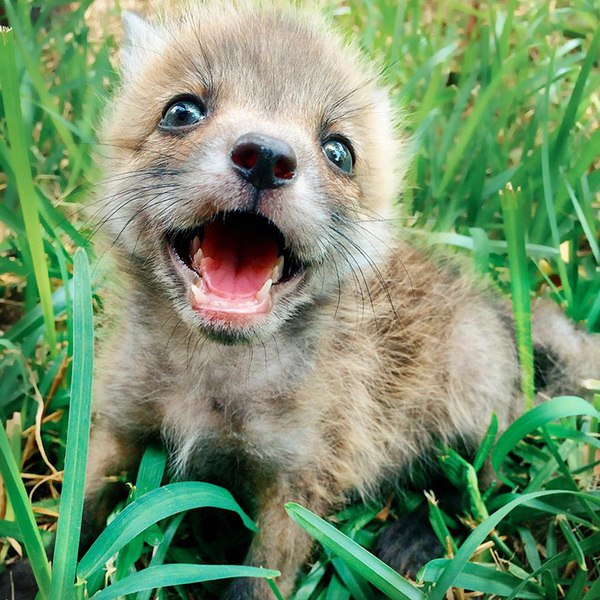
\includegraphics[width=18cm]{resources/12_decryption_result.jpg}
    \caption{Результат расшифровки сообщения}
    \label{fig:decryption-result}
\end{figure}
\section{Заключение}

В данной работе были рассмотрены некоторые практические аспекты работы с утилитой gpg. Из проведенных экспериментов можно сделать
вывод, что gpg является мощным и в то же время простым инструментом шифрования и подписи файлов. К сожалению, он не лишен недостатков 
и имеет свои <<слабые>> точки, которые, тем не менее, в большинстве своем связаны с человеческим фактором, нежели с внутренними 
деффектами данного продукта.

\end{document}